\documentclass{article}

\usepackage{graphicx} % Required for inserting images
\usepackage[
  autocite    = superscript,
  sortcites   = true,
  sorting     = none,
  style       = numeric,
  minbibnames = 3,
  ]{biblatex}

\title{\vspace{-2.5cm}Use Versalab to Observe the Photoconductivity of Vanadium oxide}
\usepackage{float} % 在导言区加入这个包

\author{Jiakang Xu}
\date{December 2024}

\addbibresource{Reference.bib}
\begin{document}

\maketitle




\section{Introduction}
In 1873 English electrical engineer Willoughby Smith discovered that the electrical resistance of selenium varies dramatically with the amount of light falling on it, which is the photoconductivity of selenium, and this is the first discovery of photoconductivity\parencite{Smith73}.The early research about Photoconductivity is limited, focused on the properties of the materials that have the photoconductivity. In the mid-20th century when semiconductor physics was developed, the understanding of photoconductivity was improved significantly. 
The research showed that the photons could excite electrons from the valence band to the conduction band in semiconductors, generating charge carriers and enhancing conductivity. And many materials like silicon, germanium, and cadmium sulfide were studied extensively for their photoconductive properties. The breakthrough of the theory then led to the development of the application. photodetectors, solar cells, and light sensors were invented. The discovery and use of polycrystalline materials and thin films expanded the scope of photoconductive technologies. Nowadays, photoconductivity is used in fields like photovoltaics, imaging technologies, and high-speed communication. 

In this experiment, we used the equipment, Versalab from Quantum Design, to observe the Photoconductivity of Vanadium oxide (VO$_{2}$) by measuring the resistance of VO$_{2}$ with laser shining on and without laser, to find out the influence of the laser to VO$_{2}$.
\section{Photoconductivity}


\\The phenomenon of photoconductivity (PC) is most clearly observed in semiconductors\parencite{boer23}. A semiconductor is a material that is between the conductor and insulator in ability to conduct. 
In conductors, apart from the completely filled energy bands, there are energy bands that are only partially filled with electrons. These bands can contribute to electrical conductivity and are referred to as conduction bands. In insulators, all energy bands except the filled bands are empty, and these empty bands lack the ability to conduct electricity. In semiconductors, there exists a series of filled bands, with the highest filled band being called the valence band, and a series of empty bands, with the lowest empty band referred to as the conduction band. Between the conduction bands and the valence bands lie bandgaps\parencite{huang1988}.

At a certain temperature or when external energy is applied, some electrons in the valence band can be excited into the conduction band, leaving positively charged electron holes in the valence band. It is also possible that impurities in the semiconductor alter the band filling, resulting in a few electrons in the conduction band and a deficiency of electrons in the valence band, creating holes. Thus, semiconductors conduct electricity through the electrons in the conduction band and the holes in the valence band. The process of the electrons in valence bands are excited to the conduction bands by the external light sources is called photoconductivity. 

%basic PC: generation+recombo rates, steady states, dark vs photocurrent

%intrinsic PC: basic explanation, some eqns.
Intrinsic PC is the process of photons are being absorbed in the valence bands and electrons are excited to the conduction bands, which creates equal numbers of electrons and holes, and is the main cause of photoconductivity in pure semiconductors, which is what we expect for our samples, VO$_{2}$.

%MORE INTRINSIC THEORY.
When the light level is changed in an intrinsic photoconductor, the generation and recombination rates shift and take from picoseconds to tens of nanoseconds to reach a new equilibrium, since intrinsic PC is insensitized. This means we can ignore transient conductivity. Consider an intrinsic photoconductor with dark conductivity $\sigma_0$. The conductivity is proportional to $\mu_nn+\mu_pp$, where n and p are carrier densities of electrons and holes, and $\mu_n$ and $\mu_p$ are their mobilities. Defining $b=\mu_n/\mu_p$, the fractional increase in conductivity due to incident light $\Delta \sigma/\sigma_0$ can be written:

\begin{equation}
    \frac{\Delta \sigma}{\sigma_0} = \frac{\sigma_f-\sigma_0}{\sigma_0} = \frac{b\Delta n+\Delta p}{bn_0+p_0}
\end{equation}

Since $\Delta p = \Delta n$ in intrinsic PC and $p=n$ for pure samples, we can write:

\begin{equation}
    \frac{\Delta \sigma}{\sigma_0} \approx \frac{\Delta n}{n_0}
\end{equation}

In terms of resistances, this can be rewritten:

\begin{equation}
    \frac{R_0}{R_f}-1\approx\frac{\Delta n}{n}
\end{equation}

which allows us to measure the fractional change due to light of charge carriers and conductivity from resistance measurements, without knowing the shape of our samples. Knowing the shape, one can measure the carrier density directly. Note that the light is in general unevenly incident along the surface of the material, so the intrinsic values given here are actually averages.


\section{Experimental Methods}
In this experiment, there are some special methods are used by us and Versalab, which make contribution to the measurements.
\subsection{4-terminal measurements}
The 4-terminal resistance measurements are one of the most common methods for a lock-in amplifier, as shown in figure~\ref{ter}(a)
They have the advantage over simpler methods with two terminals that the 4-terminal resistance measurements remove the effects of contact resistance, as shown in figure~\ref{ter}(b) and \ref{ter} (c)\parencite{Neves24}. In the 2-terminal measurement, the voltmeter measures the voltage of the whole circuit,the voltage of the lead resistance and contact resistance would be part of the measure result. However, in the 4-terminal measurements, the voltmeter is connected in parallel with the sample, so it will only measure the voltage of the sample. The measure result would not be affected by the contact resistance and lead resistance as long as the current is fixed. The Versalab uses 4-terminal measurements to obtain the more accurate resistance measurement values. As shown in the figure~\ref{pin out}, and the table~\ref{interconn}, our sample is only connected to the channel 11-14, We connect the middle two contacts of the sample to channel 13 and 14, and the outer two contacts to 11 and 12, which is the 4-terminal measurement that could remove the lead resistance and lead resistance.
\begin{figure}[H]
    \centering
    \begin{minipage}[t]{0.3\textwidth}
        \centering
        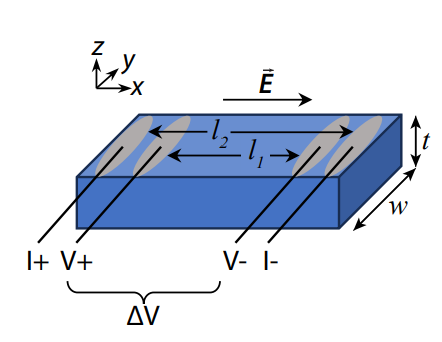
\includegraphics[width=\textwidth]{pic/4tm.png}
       \
    \end{minipage}
    \hfill
    \begin{minipage}[t]{0.3\textwidth}
        \centering
        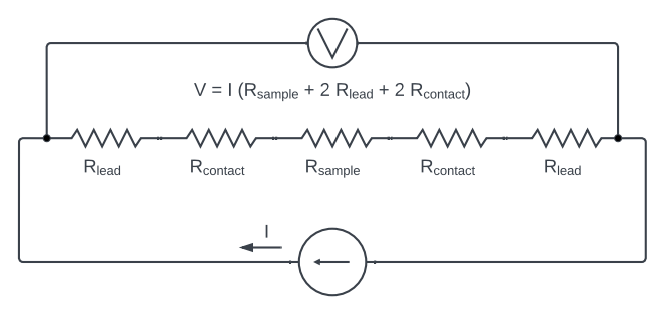
\includegraphics[width=\textwidth]{pic/2tmc.png}
    \end{minipage}
    \hfill
    \begin{minipage}[t]{0.3\textwidth}
        \centering
        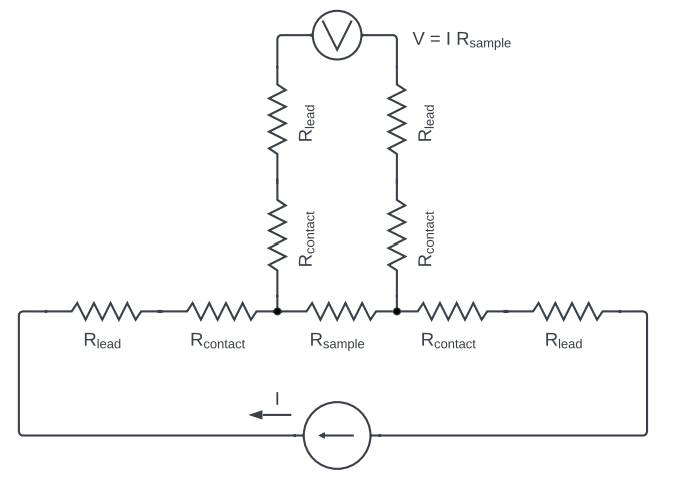
\includegraphics[width=\textwidth]{pic/4tmc.png}
    \end{minipage}
    \caption{(a) The 4-terminal measurement, (b) The 2-terminal measurement circuit, and (c) The 4-terminal measurement circuit  }
    \label{ter}
\end{figure}
\begin{figure}[H]
                \centering
                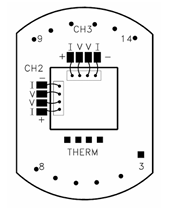
\includegraphics[width=0.25\linewidth]{4/pin out.png}
                \caption{Pin configuration of resistance bridge sample holder board}
                \label{pin out}
            \end{figure}
            \begin{table}[H]
                \centering
                \begin{tabular}{|c|c|}
                \hline
                   RESISTANCE BRIDGE & RESISTANCE BRIDGE\\
                   BOARD FUNCTION & SAMPLE HOLDER\\
                   \hline
                   Channel 1, I+ & 3    \\  \hline
                   Channel 1, I- & 4    \\  \hline
                   Channel 1, V+ & 5    \\  \hline
                   Channel 1, V- & 6    \\  \hline
                   Channel 2, I+ & 7    \\  \hline
                   Channel 2, I- & 8    \\  \hline
                   Channel 2, V+ & 9    \\  \hline
                   Channel 2, V- & 10   \\  \hline
                   Channel 3, I+ & 11   \\  \hline
                   Channel 3, I- & 12   \\  \hline
                   Channel 3, V+ & 13   \\  \hline
                   Channel 3, V- & 14   \\  \hline
                \end{tabular}
                \caption{Standard interconnection table for sample holder board}
                \label{interconn}
            \end{table}
\subsection{The thin film method}
In the measurement, we use the laser to shine on the sample. To make the sample receive more photons which could excite the electrons, we need to increase the surface area of the sample, which is the shape of thin film. We have two samples in the experiment. The first sample is a strip-shaped solid, and the second sample is a thin film. The measurements also shows that the performance of the thin film is much better than the strip-shaped solid.
\section{Sample}
\subsection{Vanadium(IV) oxide}
Vanadium(IV) oxide is an inorganic compound with the formula VO$_{2}$. It is a semiconductor at room temperature. However, the phase transition occurs around 340K, and VO$_{2}$ transfers from the monoclinic phase, which is semiconducting, to the rutile phase, which is metallic\parencite{Good71}, as the atoms in each pair separate, breaking the localized V-V bonds and releasing the bonding electrons, leading to a sharp increase in electrical conductivity\parencite{Green84}. The temperature of phase transition could be different in heating or cooling; the temperature range in heating is 335-350K, while in cooling it is 340-325K\parencite{Morin59}.The phase transition of VO$_{2}$ can occur in times as short as 100 femtoseconds, which allows it to be extremely fast optical modulators, infrared modulators for missile guidance systems, cameras, data storage, and other applications.  The optical band gap of VO2 in the semiconducting phase is about 0.7 eV\parencite{Shin90}, which is relatively low in semiconductors, meaning its has excellent conductivity.

\newpage

\printbibliography

\end{document}
